\chapter{Macchine a stati finiti (FSM)}
\label{ch:fsm}
\textit{(24 aprile 2026)}

\begin{definizione}{FSM}
\textbf{FSM} (\emph{Finite State Machine}, macchina a stati finiti): architettura in cui gli
stati presenti determinano quelli futuri. Il sistema può trovarsi in un numero finito di
stati; a ogni fronte di clock passa a uno stato futuro che dipende dallo stato presente ed,
eventualmente, dagli ingressi.
\end{definizione}

\begin{definizione}{Diagramma di stato}
mappa per rappresentare il comportamento di un sistema sequenziale (i possibili stati e i
legami fra essi). Gli stati sono legati fra loro da precise \textbf{transizioni} e sono
definiti da condizioni \textbf{interne} (presenti nel sistema) e/o da condizioni
\textbf{esterne} (segnali in ingresso dall'esterno).
\end{definizione}

\noindent Ogni circuito digitale è una FSM: un circuito che contiene $N$ flip-flop può
trovarsi al più in $2^N$ stati distinti, quindi in un numero finito di stati (un circuito
puramente combinatorio è il caso limite, con un solo stato). Per descrivere una FSM
servono cinque elementi: l'insieme degli \textbf{stati} $S_i$, gli \textbf{ingressi} $I$,
le \textbf{uscite} $O$, la \textbf{funzione di stato futuro} (come si passa da uno stato
all'altro) e la \textbf{funzione di uscita}.

% ======================================================================
\section{Tipi di architettura FSM: Moore e Mealy}

Esistono due tipi principali di architettura: \textbf{Moore} e \textbf{Mealy}. Entrambe
sono formate da tre blocchi: una logica combinatoria che calcola lo stato futuro, un
registro di memoria (i flip-flop, comandati dal clock) che conserva lo stato presente e una
logica combinatoria che genera le uscite. Le due architetture differiscono solo per
\emph{ciò che entra} nella logica delle uscite.

\subsection{Architettura di Moore}

\begin{fitcenter}
\begin{tikzpicture}[font=\small, >=latex, line width=0.6pt,
  blocco/.style={draw, thick, minimum width=2.6cm, minimum height=1.3cm, align=center, fill=noteblue!4}]
\node[blocco] (lcf) at (0,0)   {logica\\combinatoria\\stato futuro};
\node[blocco] (reg) at (4.4,0) {registro\\di memoria\\(flip-flop)};
\node[blocco] (lcu) at (8.8,0) {logica\\combinatoria\\uscite};
\draw[->] (-2.8,-0.3) -- node[below, font=\scriptsize] {ingressi $I$} ($(lcf.west)+(0,-0.3)$);
\draw[->] (lcf.east) -- node[above, font=\scriptsize] {futuro} (reg.west);
\draw[->] (reg.east) -- node[below, font=\scriptsize] {presente $Q$} (lcu.west);
\draw[->] (lcu.east) -- ++(1.4,0) node[right, font=\scriptsize] {uscite $O$};
\draw[<-] (reg.south) -- ++(0,-0.7) node[below, font=\scriptsize] {CLK};
% retroazione dello stato presente verso la logica di stato futuro
\draw[->] ($(reg.east)+(0.5,0)$) node[circle, fill, inner sep=1.2pt] {} |- (-1.9,1.3) |- ($(lcf.west)+(0,0.3)$);
\end{tikzpicture}
\end{fitcenter}

\begin{itemize}[leftmargin=1.5em, itemsep=2pt]
    \item Uno stato è univocamente conseguenza dello stato precedente (e degli ingressi, se
          ci sono): $Q^+ = f(Q, I)$. Per questo l'uscita del registro torna indietro verso
          la logica di stato futuro.
    \item Gli ingressi esterni non sempre sono presenti: un contatore o un generatore di
          sequenze, ad esempio, evolve solo al ritmo del clock.
    \item Le uscite dipendono \textbf{solo dallo stato presente}: $O = g(Q)$. Possono quindi
          cambiare solo dopo un fronte di clock (sono \textbf{sincrone}). In genere si
          tratta di più linee, cioè di un \emph{bus} di uscita.
    \item Nel diagramma di stato il valore delle uscite si scrive \textbf{dentro lo stato}.
\end{itemize}

\subsection{Architettura di Mealy}

\begin{fitcenter}
\begin{tikzpicture}[font=\small, >=latex, line width=0.6pt,
  blocco/.style={draw, thick, minimum width=2.6cm, minimum height=1.3cm, align=center, fill=noteblue!4}]
\node[blocco] (lcf) at (0,0)   {logica\\combinatoria\\stato futuro};
\node[blocco] (reg) at (4.4,0) {registro\\di memoria\\(flip-flop)};
\node[blocco] (lcu) at (8.8,0) {logica\\combinatoria\\uscite};
\draw[->] (-2.8,-0.3) -- node[above, font=\scriptsize, pos=0.3] {ingressi $I$} ($(lcf.west)+(0,-0.3)$);
\draw[->] (lcf.east) -- node[above, font=\scriptsize] {futuro} (reg.west);
\draw[->] (reg.east) -- node[below, font=\scriptsize] {presente $Q$} (lcu.west);
\draw[->] (lcu.east) -- ++(1.4,0) node[right, font=\scriptsize] {uscite $O$};
\draw[<-] (reg.south) -- ++(0,-0.7) node[below, font=\scriptsize] {CLK};
\draw[->] ($(reg.east)+(0.5,0)$) node[circle, fill, inner sep=1.2pt] {} |- (-1.9,1.3) |- ($(lcf.west)+(0,0.3)$);
% differenza rispetto a Moore: gli ingressi raggiungono anche la logica delle uscite
\draw[->, notered, thick] (-2.3,-0.3) node[circle, fill, inner sep=1.2pt] {} |- (8.8,-1.9)
      node[pos=0.75, below, font=\scriptsize] {gli ingressi entrano anche nella logica delle uscite} -- (lcu.south);
\end{tikzpicture}
\end{fitcenter}

\noindent La differenza principale fra Moore e Mealy è la dipendenza delle uscite dai
parametri del circuito:
\begin{itemize}[leftmargin=1.5em, itemsep=2pt]
    \item in \textbf{Moore}: $O_i = f(Q_i)$, uscite \textbf{sincrone} con il clock;
    \item in \textbf{Mealy}: $O_i = f(Q_i, I_i)$, uscite \textbf{asincrone}: se il clock è
          fermo ma un ingresso cambia, le uscite cambiano subito, senza aspettare il fronte.
\end{itemize}

\noindent Poiché l'uscita dipende sia dallo stato sia dall'ingresso, in Mealy il valore
delle uscite si associa alle \textbf{transizioni} e non agli stati: sulla freccia si scrive
\emph{ingresso/uscita}. Ne derivano alcune conseguenze pratiche:
\begin{itemize}[leftmargin=1.5em, itemsep=2pt]
    \item a parità di comportamento, Mealy richiede in genere \textbf{meno stati} (e quindi
          meno flip-flop) di Moore;
    \item Mealy \textbf{reagisce prima}: l'uscita risponde all'ingresso nello stesso periodo
          di clock, mentre Moore risponde dopo il fronte successivo;
    \item in Mealy eventuali glitch sugli ingressi si propagano direttamente alle uscite;
          in Moore le uscite restano stabili per tutto il periodo di clock.
\end{itemize}
Gli esempi delle sezioni successive mostrano la stessa macchina realizzata in entrambi i modi.

% ======================================================================
\section{Dal diagramma di stato al circuito}

Il diagramma di stato è composto da \textbf{stati} (cerchi, che in una macchina di Moore
riportano anche il valore delle uscite) collegati da \textbf{transizioni} (frecce, su cui si
scrive la condizione sugli ingressi che le attiva). Come esempio si considera una macchina
di Moore senza ingressi che percorre ciclicamente tre stati, con tre uscite $O_2O_1O_0$:

\begin{center}
\begin{tikzpicture}[font=\small, >=latex, line width=0.6pt,
  stato/.style={draw, circle, thick, minimum size=1.25cm, align=center, inner sep=1pt}]
\node[stato] (s0) at (0,1.6)     {$S_0$\\[-2pt]\footnotesize 010};
\node[stato] (s1) at (2.0,-0.6)  {$S_1$\\[-2pt]\footnotesize 011};
\node[stato] (s2) at (-2.0,-0.6) {$S_2$\\[-2pt]\footnotesize 101};
\draw[->] (s0) to[bend left=20] (s1);
\draw[->] (s1) to[bend left=20] node[below, font=\scriptsize, color=noteteal] (tr) {transizione} (s2);
\draw[->] (s2) to[bend left=20] (s0);
\node[font=\scriptsize, color=noteteal, anchor=west] (lst) at (1.6,2.3) {stato};
\draw[->, noteteal, thin] (lst.west) -- (s0.north east);
\node[font=\scriptsize, color=noteteal, anchor=west] (lv) at (3.2,0.4) {valore di uscita $O_2O_1O_0$};
\draw[->, noteteal, thin] (lv.south west) -- (s1.north east);
\end{tikzpicture}
\end{center}

\noindent La procedura per passare dal diagramma di stato al circuito è la seguente.

\begin{enumerate}[leftmargin=1.8em, itemsep=4pt, label=\textbf{\arabic*)}]
    \item \textbf{Dato il numero di stati} (3), definisco il numero di bit che mi serve a
          rappresentarli: il più piccolo $n$ tale che $2^n \ge 3$, cioè
          $n = \lceil \log_2 3 \rceil = 2$ bit.
    \item \textbf{Associo a ogni stato una rappresentazione in bit}:
          $S_0=[00]$, $S_1=[01]$, $S_2=[10]$. La combinazione avanzata $[11]$ non
          corrisponde ad alcuno stato: è un \emph{don't care} ($\times$).
    \item \textbf{Per ogni bit uso un FF}: lo stato è la coppia $Q_1Q_0$ memorizzata da due
          flip-flop.
    \item \textbf{Scrivo la tabella di verità} (tabella delle transizioni): associo a ogni
          stato presente $Q_1Q_0$ lo stato futuro $Q_1^+Q_0^+$.
\begin{center}
\begin{tabular}{c|cc|cc}
\toprule
Stato & $Q_1$ & $Q_0$ & $Q_1^+$ & $Q_0^+$ \\
\midrule
$S_0$ & 0 & 0 & 0 & 1 \\
$S_1$ & 0 & 1 & 1 & 0 \\
$S_2$ & 1 & 0 & 0 & 0 \\
--    & 1 & 1 & $\times$ & $\times$ \\
\bottomrule
\end{tabular}
\end{center}
    \item \textbf{Scelgo il tipo di FF} (D, JK, T). In questo caso uso i DFF: poiché
          $Q_i^+ = D_i$, le colonne degli ingressi $D_i$ coincidono con quelle dello stato
          futuro.
    \item \textbf{Ricavo le funzioni $D_i = f(Q_i)$}, sfruttando il don't care:
          \begin{itemize}[leftmargin=1.2em]
              \item $D_1$ vale 1 solo per $Q_1Q_0=01$; ponendo a 1 anche il don't care $11$
                    si raggruppano le due righe con $Q_0=1$: $D_1 = Q_0$;
              \item $D_0$ vale 1 solo per $Q_1Q_0=00$, che non è adiacente a $11$:
                    $D_0 = \overline{Q_1}\cdot\overline{Q_0} = \overline{Q_1+Q_0}$ (una NOR).
          \end{itemize}
    \item \textbf{Disegno il circuito} della logica di stato futuro e del registro (lo
          schema completo, con la logica delle uscite, è riportato al termine della
          procedura).
    \item \textbf{Trovo le funzioni dei segnali di uscita $O_i = f(Q_i)$}, leggendo il
          valore di uscita scritto in ciascuno stato:
\begin{center}
\begin{tabular}{cc|cc|ccc}
\toprule
$Q_1$ & $Q_0$ & $D_1$ & $D_0$ & $O_2$ & $O_1$ & $O_0$ \\
\midrule
0 & 0 & 0 & 1 & 0 & 1 & 0 \\
0 & 1 & 1 & 0 & 0 & 1 & 1 \\
1 & 0 & 0 & 0 & 1 & 0 & 1 \\
1 & 1 & $\times$ & $\times$ & $\times$ & $\times$ & $\times$ \\
\bottomrule
\end{tabular}
\qquad
$\begin{aligned}
O_0 &= Q_0 + Q_1 \\
O_1 &= \overline{Q_1} \\
O_2 &= Q_1
\end{aligned}$
\end{center}
    \item \textbf{Verifico lo stato futuro della combinazione non usata}
          $Q_1=Q_0=1$: se fosse uno \textbf{stato bloccante} sarebbe un problema da
          risolvere (vedi più avanti).
\end{enumerate}

\noindent Il circuito completo realizza i tre blocchi dell'architettura di Moore: la NOR
e il collegamento $Q_0\to D_1$ formano la logica di stato futuro, i due DFF il registro, la
porta OR e i collegamenti diretti la logica delle uscite.

\begin{fitcenter}
\begin{circuitikz}[line width=0.6pt, font=\small, >=latex]
\ctikzset{flipflops/scale=0.85}
\node[flipflop D] (FF0) at (0,0) {};
\node[flipflop D] (FF1) at (3.6,0) {};
\node[font=\scriptsize, below] at (FF0.south) {FF$_0$};
\node[font=\scriptsize, below] at (FF1.south) {FF$_1$};
% Q0 -> D1
\draw (FF0.pin 6) -- (FF1.pin 1);
\node[font=\scriptsize, above] at ($(FF0.pin 6)+(0.35,0)$) {$Q_0$};
% NOR di stato futuro: D0 = not(Q1 + Q0)
\node[nor port, xscale=-1] (NR) at (-0.6,2.5) {};
\node[font=\scriptsize, above] at (NR.north) {$D_0=\overline{Q_1+Q_0}$};
\draw (NR.out) -- ++(-0.5,0) coordinate (no) -- (no |- FF0.pin 1) -- (FF0.pin 1);
\draw (FF0.pin 6) ++(0.85,0) node[circle, fill, inner sep=1.1pt] {} coordinate (q0) -- (q0 |- 0,3.4);
\node[circle, fill, inner sep=1.1pt] at (q0 |- NR.in 2) {};
\draw (q0 |- NR.in 2) -- (NR.in 2);
\draw (FF1.pin 6) -- ++(0.7,0) coordinate (q1) node[circle, fill, inner sep=1.1pt] {};
\node[jump crossing] (JX) at (q0 |- NR.in 1) {};
\draw (q1) |- (JX.east);
\draw (JX.west) -- (NR.in 1);
% logica delle uscite
\node[or port] (OR) at (7.6,2.0) {};
\draw (q0 |- 0,3.4) -| ($(OR.in 1)+(-1.1,0)$) |- (OR.in 1);
\node[circle, fill, inner sep=1.1pt] at (q1 |- OR.in 2) {};
\draw (q1 |- OR.in 2) -- (OR.in 2);
\draw[->] (OR.out) -- (9.4,0 |- OR.out) node[right, font=\scriptsize] {$O_0$};
\draw[->] (q1) -- (9.4,0 |- q1) node[right, font=\scriptsize] {$O_2$};
\draw[->] (FF1.pin 4) -- (9.4,0 |- FF1.pin 4) node[right, font=\scriptsize] {$O_1$};
\node[font=\scriptsize, above] at ($(FF1.pin 6)+(0.35,0)$) {$Q_1$};
\node[font=\scriptsize, below] at ($(FF1.pin 4)+(0.45,0)$) {$\overline{Q_1}$};
% clock comune
\draw (FF0.pin 3) -- ++(-0.3,0) coordinate (c0) -- (c0 |- 0,-1.8);
\draw (FF1.pin 3) -- ++(-0.3,0) coordinate (c1) -- (c1 |- 0,-1.8);
\draw (-1.9,-1.8) node[left, font=\scriptsize] {CLK} -- (c1 |- 0,-1.8);
\node[circle, fill, inner sep=1.1pt] at (c0 |- 0,-1.8) {};
\end{circuitikz}
\end{fitcenter}

\begin{important}
\textbf{Scelta del tipo di flip-flop.}
\begin{itemize}[leftmargin=1.3em, itemsep=2pt]
    \item \textbf{DFF}: $Q^+ = D$. È il più usato e il più semplice: l'ingresso da
          calcolare coincide con lo stato futuro.
    \item \textbf{TFF}: $Q^+ = T\oplus Q$. Adatto a contatori e sequenze regolari: $T=1$ solo
          quando il bit deve cambiare.
    \item \textbf{JKFF}: $Q^+ = J\overline{Q}+\overline{K}Q$. Flessibile, può fare tutto
          (set, reset, toggle, hold).
\end{itemize}
Per ricavare gli ingressi dei FF dalla tabella delle transizioni si usa la
\textbf{tabella di eccitazione}, che indica quale ingresso produce ciascun passaggio
$Q \to Q^+$:
\begin{center}
\begin{tabular}{c|c|c|cc}
\toprule
$Q \to Q^+$ & $D$ & $T$ & $J$ & $K$ \\
\midrule
$0 \to 0$ & 0 & 0 & 0 & $\times$ \\
$0 \to 1$ & 1 & 1 & 1 & $\times$ \\
$1 \to 0$ & 0 & 1 & $\times$ & 1 \\
$1 \to 1$ & 1 & 0 & $\times$ & 0 \\
\bottomrule
\end{tabular}
\end{center}
\end{important}

\subsection{Stato bloccante}

Al punto 9 si verifica quale sia lo stato futuro della combinazione non usata
$Q_1=Q_0=1$. Uno \textbf{stato bloccante} è uno stato non previsto dal quale la macchina non
torna più nel ciclo principale (ad esempio perché $11 \to 11$): se all'accensione, o per un
disturbo, i flip-flop finissero in quello stato, il circuito resterebbe fermo. È un problema
che dobbiamo risolvere, assegnando esplicitamente uno stato futuro alla combinazione non
usata (invece di lasciarla don't care) oppure prevedendo un reset.

\noindent Nel nostro caso, da $Q=11$ si ottiene $D_1=Q_0=1$ e
$D_0=\overline{Q_1}\,\overline{Q_0}=0$: si va a finire in $10=S_2$, quindi la sequenza
ricomincia e il circuito non si blocca.

\subsection{Segnale di Enable: percorrere il ciclo nei due versi}

Se volessimo scorrere il ciclo anche al contrario, possiamo inserire un ingresso di
\textbf{Enable} $E$ che sceglie il verso:
\begin{itemize}[leftmargin=1.5em, itemsep=1pt]
    \item $E=1$: $010 \to 011 \to 101$, cioè $S_0\to S_1\to S_2\to S_0$ (verso diritto,
          frecce tratteggiate);
    \item $E=0$: $101 \to 011 \to 010$, cioè $S_2\to S_1\to S_0\to S_2$ (verso rovescio,
          frecce continue).
\end{itemize}

\begin{center}
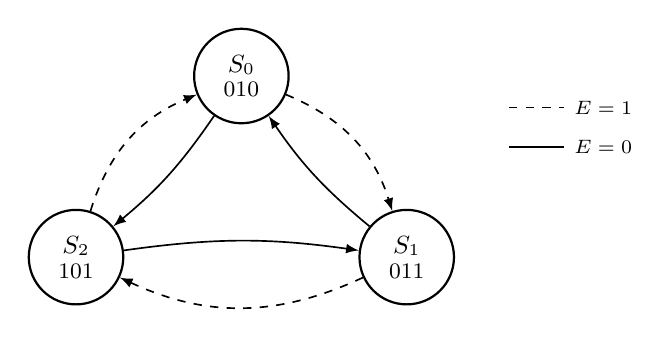
\begin{tikzpicture}[font=\small, >=latex, line width=0.6pt,
  stato/.style={draw, circle, thick, minimum size=1.2cm, align=center, inner sep=1pt}]
\node[stato] (s0) at (0,1.7)     {$S_0$\\[-2pt]\footnotesize 010};
\node[stato] (s1) at (2.1,-0.6)  {$S_1$\\[-2pt]\footnotesize 011};
\node[stato] (s2) at (-2.1,-0.6) {$S_2$\\[-2pt]\footnotesize 101};
\draw[->, dashed] (s0) to[bend left=25] (s1);
\draw[->, dashed] (s1) to[bend left=25] (s2);
\draw[->, dashed] (s2) to[bend left=25] (s0);
\draw[->] (s0) to[bend left=8] (s2);
\draw[->] (s2) to[bend left=8] (s1);
\draw[->] (s1) to[bend left=8] (s0);
\draw[dashed] (3.4,1.3) -- ++(0.7,0) node[right, font=\scriptsize] {$E=1$};
\draw (3.4,0.8) -- ++(0.7,0) node[right, font=\scriptsize] {$E=0$};
\end{tikzpicture}
\end{center}

\noindent Cambiano gli ingressi dei flip-flop, ma le uscite restano le stesse: l'ingresso
$E$ entra solo nella logica di stato futuro, quindi la macchina è ancora di Moore.
\[
D_i = f(Q_i, E) \qquad\qquad O_i = f(Q_i)
\]

\begin{center}
\begin{tabular}{c|cc|cc}
\toprule
$E$ & $Q_1$ & $Q_0$ & $D_1=Q_1^+$ & $D_0=Q_0^+$ \\
\midrule
0 & 0 & 0 & 1 & 0 \\
0 & 0 & 1 & 0 & 0 \\
0 & 1 & 0 & 0 & 1 \\
0 & 1 & 1 & $\times$ & $\times$ \\
\midrule
1 & 0 & 0 & 0 & 1 \\
1 & 0 & 1 & 1 & 0 \\
1 & 1 & 0 & 0 & 0 \\
1 & 1 & 1 & $\times$ & $\times$ \\
\bottomrule
\end{tabular}
\end{center}

\noindent Dalla tabella possiamo scrivere le funzioni:
\[
D_1 = \overline{E}\cdot\overline{Q_1}\cdot\overline{Q_0} + E\cdot Q_0
\qquad\qquad
D_0 = E\cdot\overline{Q_1}\cdot\overline{Q_0} + \overline{E}\cdot Q_1
\]
Ripetendo la verifica del punto 9: da $Q=11$ si va in $10=S_2$ se $E=1$ e in $01=S_1$ se
$E=0$; in entrambi i casi la combinazione non usata non è bloccante.

\begin{fitcenter}
\begin{tikzpicture}[font=\small, >=latex, line width=0.6pt,
  blocco/.style={draw, thick, minimum height=1.6cm, align=center, fill=noteblue!4}]
\node[blocco, minimum width=2.8cm] (lf) at (0,0) {logica che permette\\di ottenere\\$D_i=f(Q_i,E)$};
\node[blocco, minimum width=2.2cm] (rg) at (4.3,0) {2 DFF};
\node[blocco, minimum width=2.8cm] (lu) at (8.6,0) {logica che permette\\di ottenere\\$O_i=f(Q_i)$};
\draw[->, very thick] (lf.east) -- node[below, font=\scriptsize] {$D_1D_0$} (rg.west);
\draw[->, very thick] (rg.east) -- node[below, font=\scriptsize, pos=0.7] {$Q_1Q_0$} (lu.west);
\draw[->, very thick] (lu.east) -- ++(1.3,0) node[right, font=\scriptsize] {$O_2O_1O_0$};
\draw[->] (-2.6,-0.35) node[left, font=\scriptsize] {$E$} -- ($(lf.west)+(0,-0.35)$);
\draw[<-] (rg.south) -- ++(0,-0.8) node[below, font=\scriptsize] {CLK};
\draw[->, very thick] ($(rg.east)!0.35!(lu.west)$) node[circle, fill, inner sep=1.6pt] {}
      |- (-2.0,1.5) node[pos=0.75, above, font=\scriptsize] {stato presente $Q_1Q_0$}
      |- ($(lf.west)+(0,0.35)$);
\end{tikzpicture}
\end{fitcenter}

% ======================================================================
\section{Esempio: insegna luminosa}
\textit{(27 aprile 2026)}

\tikzset{
  stato/.style={draw, circle, thick, minimum size=1.2cm, align=center, inner sep=1pt},
  etich/.style={font=\scriptsize, fill=white, inner sep=1pt}
}

Un'insegna luminosa ha due lampade, \textbf{R} (rossa) e \textbf{B} (blu), e un ingresso di
abilitazione $E$. Indicando con A = accesa e S = spenta:
\[
R_AB_A \to R_AB_S \to R_SB_A \to R_AB_A \to \cdots \qquad (E=1)
\]
\[
B_A \to B_S \to B_A \to \cdots \quad\text{con } R \text{ sempre spenta} \qquad (E=0)
\]
Con $E=1$ l'insegna percorre tre configurazioni (entrambe accese, solo R, solo B); con
$E=0$ la lampada rossa resta spenta e la blu lampeggia.

\subsection{Soluzione con Moore}

Con $E=1$ bastano tre stati, ciascuno con la propria uscita: $S_0=[RB]$, $S_1=[R]$,
$S_2=[B]$ (diagramma a sinistra). Per il funzionamento con $E=0$ serve però una
configurazione con \emph{entrambe} le lampade spente, che non corrisponde a nessuno dei tre
stati. In Moore le uscite dipendono solo dallo stato ($O_i = f(Q_i)$, e non da $E$),
quindi per aggiungere questa configurazione \textbf{dobbiamo aggiungere un 4° stato}
$S_3=[-]$ (diagramma a destra).

\begin{fitcenter}
\begin{tikzpicture}[>=latex, line width=0.6pt, font=\small]
% ciclo con E=1 (3 stati)
\node[stato] (a0) at (0,1.8)    {$S_0$\\[-2pt]\footnotesize [RB]};
\node[stato] (a1) at (-1.6,-0.6) {$S_1$\\[-2pt]\footnotesize [R]};
\node[stato] (a2) at (1.6,-0.6)  {$S_2$\\[-2pt]\footnotesize [B]};
\draw[->, dashed] (a0) to[bend right=20] (a1);
\draw[->, dashed] (a1) to[bend right=20] (a2);
\draw[->, dashed] (a2) to[bend right=20] (a0);
\node[font=\footnotesize] at (0,-2.2) {solo $E=1$ (3 stati)};
% diagramma completo (4 stati)
\begin{scope}[xshift=7.2cm]
\node[stato] (s0) at (0,2.2)   {$S_0$\\[-2pt]\footnotesize [RB]};
\node[stato] (s1) at (-2.3,0)  {$S_1$\\[-2pt]\footnotesize [R]};
\node[stato] (s2) at (2.3,0)   {$S_2$\\[-2pt]\footnotesize [B]};
\node[stato] (s3) at (0,-2.2)  {$S_3$\\[-2pt]\footnotesize [--]};
% E = 1
\draw[->, dashed] (s0) to[bend right=15] (s1);
\draw[->, dashed] (s1) -- (s2);
\draw[->, dashed] (s2) to[bend right=15] (s0);
% E = 0
\draw[->] (s0.west) .. controls (-4.2,2.6) and (-4.2,-2.6) .. (s3.west);
\draw[->] (s1) to[bend right=15] (s3);
\draw[->] (s2) to[bend left=20] (s3);
% da S3 si va in S2 per qualsiasi E
\draw[->, notered, thick] (s3) to[bend left=20] (s2);
\node[font=\scriptsize, text=notered, anchor=west] at (1.9,-1.6) {$E=0$ oppure $1$};
\node[font=\footnotesize] at (0,-3.6) {diagramma completo (4 stati)};
\end{scope}
\draw[dashed] (10.4,2.6) -- ++(0.6,0) node[right, font=\scriptsize] {$E=1$};
\draw (10.4,2.1) -- ++(0.6,0) node[right, font=\scriptsize] {$E=0$};
\end{tikzpicture}
\end{fitcenter}

\noindent Lettura del diagramma completo:
\begin{itemize}[leftmargin=1.5em, itemsep=1pt]
    \item con $E=1$ (tratteggiate) si percorre $S_0 \to S_1 \to S_2 \to S_0$; se ci si
          trova in $S_3$ si rientra nel ciclo passando per $S_2$;
    \item con $E=0$ (continue) da qualunque stato si va in $S_3$ (tutto spento), e poi si
          alterna $S_3 \to S_2 \to S_3$: la blu lampeggia e la rossa resta spenta.
\end{itemize}

\noindent Codificando $S_0=00$, $S_1=01$, $S_2=10$, $S_3=11$ si ottiene la tabella (si
usano DFF, quindi $D_i=Q_i^+$):

\begin{center}
\begin{tabular}{c|cc|cc|cc}
\toprule
$E$ & $Q_1$ & $Q_0$ & $D_1$ & $D_0$ & $R$ & $B$ \\
\midrule
0 & 0 & 0 & 1 & 1 & 1 & 1 \\
0 & 0 & 1 & 1 & 1 & 1 & 0 \\
0 & 1 & 0 & 1 & 1 & 0 & 1 \\
0 & 1 & 1 & 1 & 0 & 0 & 0 \\
\midrule
1 & 0 & 0 & 0 & 1 & 1 & 1 \\
1 & 0 & 1 & 1 & 0 & 1 & 0 \\
1 & 1 & 0 & 0 & 0 & 0 & 1 \\
1 & 1 & 1 & 1 & 0 & 0 & 0 \\
\bottomrule
\end{tabular}
\end{center}

\noindent Le uscite dipendono solo da $Q_1Q_0$ e risultano semplicissime, mentre la logica
di stato futuro dipende anche da $E$:
\[
R = \overline{Q_1} \qquad B = \overline{Q_0} \qquad
D_1 = \overline{E} + Q_0 \qquad
D_0 = \overline{Q_1}\,\overline{Q_0} + \overline{E}\,\overline{Q_1} + \overline{E}\,\overline{Q_0}
\]
Tutte le 4 combinazioni sono usate, quindi non ci sono stati bloccanti.

\subsection{Soluzione con Mealy}

Con Mealy le uscite possono dipendere anche da $E$, quindi la configurazione ``tutto
spento'' non richiede uno stato dedicato: bastano \textbf{3 stati} ($S_0=00$, $S_1=01$,
$S_2=10$) e il valore delle uscite si scrive sulle transizioni, nella forma $E/$uscita.

\begin{center}
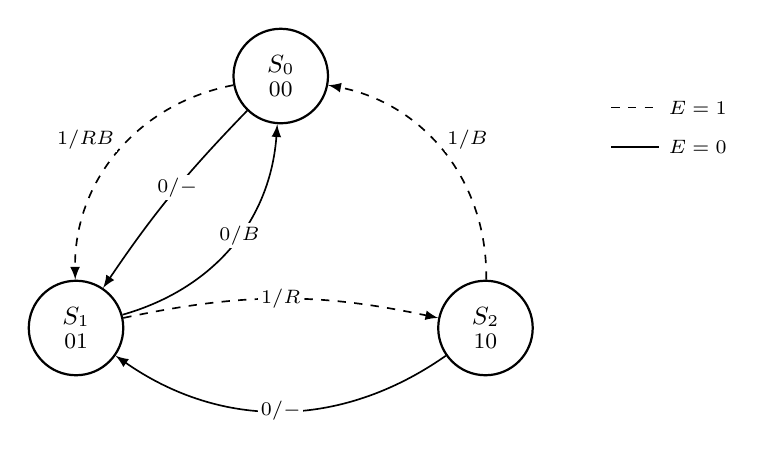
\begin{tikzpicture}[>=latex, line width=0.6pt, font=\small]
\node[stato] (s0) at (0,2.2)    {$S_0$\\[-2pt]\footnotesize 00};
\node[stato] (s1) at (-2.6,-1.0) {$S_1$\\[-2pt]\footnotesize 01};
\node[stato] (s2) at (2.6,-1.0)  {$S_2$\\[-2pt]\footnotesize 10};
% E = 1 (tratteggiate)
\draw[->, dashed] (s0) to[bend right=40] node[etich, above left] {$1/RB$} (s1);
\draw[->, dashed] (s1) to[bend left=12] node[etich] {$1/R$} (s2);
\draw[->, dashed] (s2) to[bend right=40] node[etich, above right] {$1/B$} (s0);
% E = 0 (continue)
\draw[->] (s0) to[bend right=5] node[etich, pos=0.45] {$0/-$} (s1);
\draw[->] (s1) to[bend right=35] node[etich, pos=0.55] {$0/B$} (s0);
\draw[->] (s2) to[bend left=35] node[etich] {$0/-$} (s1);
\draw[dashed] (4.2,1.8) -- ++(0.6,0) node[right, font=\scriptsize] {$E=1$};
\draw (4.2,1.3) -- ++(0.6,0) node[right, font=\scriptsize] {$E=0$};
\end{tikzpicture}
\end{center}

\noindent Con $E=1$ il ciclo $S_0\to S_1\to S_2\to S_0$ produce le uscite $RB$, $R$, $B$;
con $E=0$ la macchina alterna $S_0 \to S_1 \to S_0$ producendo $-$, $B$, $-$, \ldots\ (da
$S_2$ si rientra in $S_1$). L'uscita è quindi legata al \emph{passaggio} fra due stati e non
allo stato di per sé. Per questo è asincrona: dipende anche da $E$, che può cambiare in
qualsiasi istante; se il clock si ferma ma $E$ cambia, le uscite cambiano.

\subsubsection*{Tabella delle transizioni e delle uscite}

\begin{center}
\begin{tabular}{c|cc|cc|cc}
\toprule
 & & & \multicolumn{2}{c|}{stato futuro} & \multicolumn{2}{c}{uscite} \\
$E$ & $Q_1$ & $Q_0$ & $Q_1^+$ & $Q_0^+$ & $R$ & $B$ \\
\midrule
1 & 0 & 0 & 0 & 1 & 1 & 1 \\
1 & 0 & 1 & 1 & 0 & 1 & 0 \\
1 & 1 & 0 & 0 & 0 & 0 & 1 \\
1 & 1 & 1 & $\times$ & $\times$ & $\times$ & $\times$ \\
\midrule
0 & 0 & 0 & 0 & 1 & 0 & 0 \\
0 & 0 & 1 & 0 & 0 & 0 & 1 \\
0 & 1 & 0 & 0 & 1 & 0 & 0 \\
0 & 1 & 1 & $\times$ & $\times$ & $\times$ & $\times$ \\
\bottomrule
\end{tabular}
\end{center}

\noindent Dalla tabella si ricavano direttamente le funzioni di stato futuro e di uscita
(usando i don't care):
\[
Q_1^+ = E\,Q_0 \qquad Q_0^+ = \overline{Q_0}\,(\overline{E}+\overline{Q_1})
\qquad\qquad R = E\,\overline{Q_1} \qquad B = E \oplus Q_0
\]
Le uscite contengono $E$: è proprio ciò che caratterizza la macchina di Mealy.

\subsubsection*{Implementazione con JKFF in modalità toggle/hold}

Per implementare il registro si usano JKFF con gli ingressi \textbf{collegati insieme}
($J=K$): in questo modo il flip-flop ha solo due modalità, \textbf{toggle} ($J=K=1$,
$Q^+=\overline{Q}$) oppure \textbf{hold} ($J=K=0$, $Q^+=Q$), e si comporta come un TFF.
L'ingresso $JK_i$ vale quindi $JK_i = Q_i \oplus Q_i^+$:
\begin{itemize}[leftmargin=1.5em, itemsep=1pt]
    \item quando $Q_i = Q_i^+$ il FF deve fare \textbf{hold}: $JK_i=0$;
    \item quando $\overline{Q_i} = Q_i^+$ il FF deve fare \textbf{toggle}: $JK_i=1$.
\end{itemize}

\begin{center}
\begin{tabular}{c|cc|cc|cc}
\toprule
$E$ & $Q_1$ & $Q_0$ & $Q_1^+$ & $Q_0^+$ & $JK_1$ & $JK_0$ \\
\midrule
1 & 0 & 0 & 0 & 1 & 0 & 1 \\
1 & 0 & 1 & 1 & 0 & 1 & 1 \\
1 & 1 & 0 & 0 & 0 & 1 & 0 \\
1 & 1 & 1 & $\times$ & $\times$ & $\times$ & $\times$ \\
\midrule
0 & 0 & 0 & 0 & 1 & 0 & 1 \\
0 & 0 & 1 & 0 & 0 & 0 & 1 \\
0 & 1 & 0 & 0 & 1 & 1 & 1 \\
0 & 1 & 1 & $\times$ & $\times$ & $\times$ & $\times$ \\
\bottomrule
\end{tabular}
\end{center}

\subsubsection*{Mappe di Karnaugh per $JK_0$ e $JK_1$}

Le righe della mappa sono i valori di $E$, le colonne i valori di $Q_1Q_0$ in codice Gray (stessa tecnica di semplificazione della \cref{sec:karnaugh}).

\begin{fitcenter}
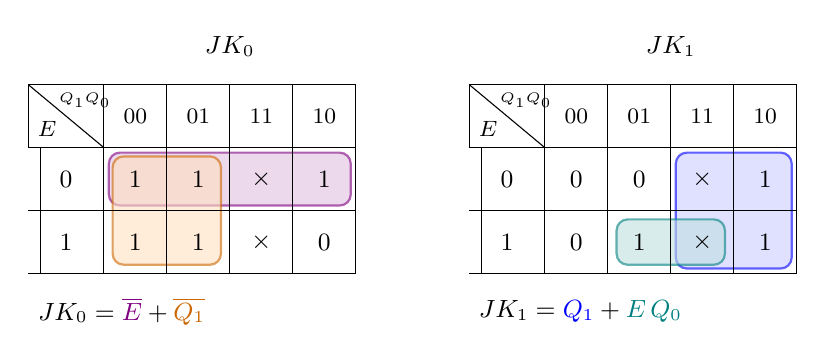
\begin{tikzpicture}[scale=0.8, font=\small]
% ---------- JK0 ----------
\begin{scope}
\node[font=\small\bfseries] at (2,3.6) {$JK_0$};
\draw[rounded corners, fill=violet!25, opacity=0.6, draw=violet, thick] (0.08,1.08) rectangle (3.92,1.92);
\draw[rounded corners, fill=orange!25, opacity=0.6, draw=orange!80!black, thick] (0.14,0.14) rectangle (1.86,1.86);
\draw (0,0) grid (4,2);
\draw (0,2) grid (4,3);
\draw (-1.2,0) grid (0,2);
\draw (-1.2,2) rectangle (0,3);
\draw (-1.2,3) -- (0,2);
\node[font=\footnotesize] at (-0.9,2.3) {$E$};
\node[font=\tiny] at (-0.3,2.75) {$Q_1Q_0$};
\foreach \c/\t in {0/00, 1/01, 2/11, 3/10}{ \node[font=\footnotesize] at (\c+0.5,2.5) {\t}; }
\node at (-0.6,1.5) {0}; \node at (-0.6,0.5) {1};
\node at (0.5,1.5) {1}; \node at (1.5,1.5) {1}; \node at (2.5,1.5) {$\times$}; \node at (3.5,1.5) {1};
\node at (0.5,0.5) {1}; \node at (1.5,0.5) {1}; \node at (2.5,0.5) {$\times$}; \node at (3.5,0.5) {0};
\node[anchor=west] at (-1.2,-0.6) {$JK_0 = \textcolor{violet}{\overline{E}} + \textcolor{orange!80!black}{\overline{Q_1}}$};
\end{scope}
% ---------- JK1 ----------
\begin{scope}[xshift=7cm]
\node[font=\small\bfseries] at (2,3.6) {$JK_1$};
\draw[rounded corners, fill=blue!20, opacity=0.6, draw=blue, thick] (2.08,0.08) rectangle (3.92,1.92);
\draw[rounded corners, fill=teal!25, opacity=0.6, draw=teal, thick] (1.14,0.14) rectangle (2.86,0.86);
\draw (0,0) grid (4,2);
\draw (0,2) grid (4,3);
\draw (-1.2,0) grid (0,2);
\draw (-1.2,2) rectangle (0,3);
\draw (-1.2,3) -- (0,2);
\node[font=\footnotesize] at (-0.9,2.3) {$E$};
\node[font=\tiny] at (-0.3,2.75) {$Q_1Q_0$};
\foreach \c/\t in {0/00, 1/01, 2/11, 3/10}{ \node[font=\footnotesize] at (\c+0.5,2.5) {\t}; }
\node at (-0.6,1.5) {0}; \node at (-0.6,0.5) {1};
\node at (0.5,1.5) {0}; \node at (1.5,1.5) {0}; \node at (2.5,1.5) {$\times$}; \node at (3.5,1.5) {1};
\node at (0.5,0.5) {0}; \node at (1.5,0.5) {1}; \node at (2.5,0.5) {$\times$}; \node at (3.5,0.5) {1};
\node[anchor=west] at (-1.2,-0.6) {$JK_1 = \textcolor{blue}{Q_1} + \textcolor{teal}{E\,Q_0}$};
\end{scope}
\end{tikzpicture}
\end{fitcenter}

\begin{itemize}[leftmargin=1.5em, itemsep=2pt]
    \item $JK_0$: la riga $E=0$ è tutta a 1 (con il don't care) e dà $\overline{E}$; le
          colonne $00$ e $01$ sono a 1 in entrambe le righe e danno $\overline{Q_1}$.
    \item $JK_1$: le colonne $11$ e $10$ (con i don't care) danno $Q_1$; la coppia
          $E=1$, $Q_1Q_0\in\{01, 11\}$ dà $E\,Q_0$.
\end{itemize}

\begin{important}
\textbf{Moore o Mealy per l'insegna?}
\begin{itemize}[leftmargin=1.3em, itemsep=2pt]
    \item \textbf{Moore}: 4 stati, uscite molto semplici ($R=\overline{Q_1}$,
          $B=\overline{Q_0}$) e sincrone; le lampade cambiano solo sul fronte di clock.
    \item \textbf{Mealy}: 3 stati, ma le uscite dipendono da $E$ ($R=E\,\overline{Q_1}$,
          $B=E\oplus Q_0$): un cambiamento di $E$ si vede subito sulle lampade, anche a
          clock fermo.
\end{itemize}
\end{important}

% ======================================================================
\section{Esempio: riconoscitore di sequenze}

In ingresso arriva una serie di bit $I$, uno per ogni periodo di clock: vogliamo accendere
un LED quando troviamo \textbf{due 1 consecutivi} ($I_{i+1}I_i=11$). Le coppie possono
sovrapporsi: in $111$ ci sono due coppie.
\[
I = 1\;0\;\mathbf{1\;1}\;0\;1\;0\;\mathbf{1\;1\;1}\;0\;0\;0\;1\;\ldots
\]
In questa serie le coppie di 1 consecutivi sono tre (3°--4° bit, 8°--9° bit e 9°--10° bit),
quindi il LED deve accendersi tre volte.

\noindent Per Moore servono tre stati:
\begin{itemize}[leftmargin=1.5em, itemsep=1pt]
    \item $S_0$ = non ho ancora trovato il 1° 1: LED spento (S);
    \item $S_1$ = ho trovato il 1° 1: LED spento (S);
    \item $S_2$ = ho trovato il 2° 1: LED acceso (A).
\end{itemize}
Con Mealy bastano due stati, perché il LED si può accendere direttamente sulla
transizione: $S_0$ = l'ultimo bit ricevuto è 0, $S_1$ = l'ultimo bit ricevuto è 1.
Nei diagrammi le frecce tratteggiate corrispondono a $I=1$, quelle continue a $I=0$; nel
diagramma di Mealy le transizioni riportano $I$/LED.

\begin{fitcenter}
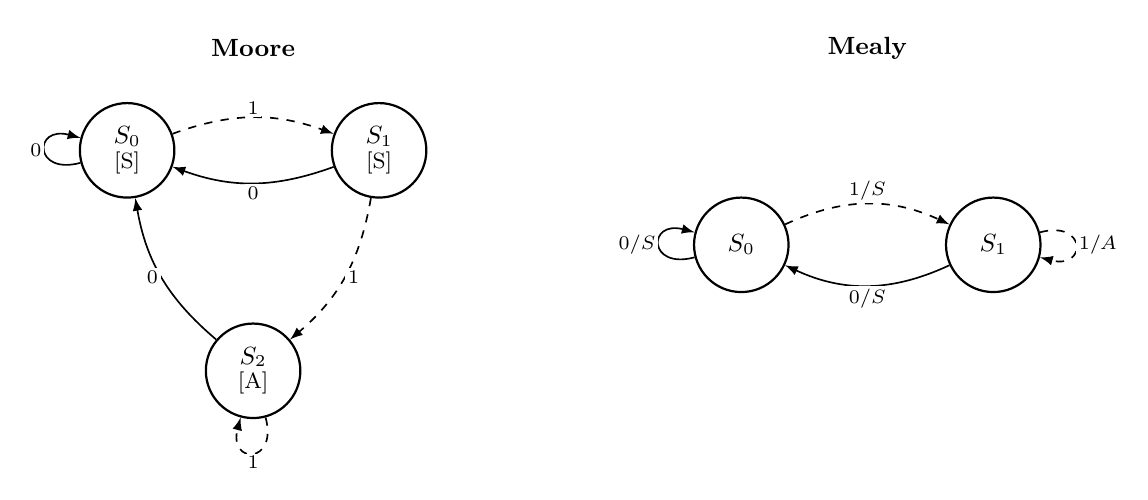
\begin{tikzpicture}[>=latex, line width=0.6pt, font=\small]
% ---------- Moore ----------
\node[stato] (m0) at (0,0)      {$S_0$\\[-2pt]\footnotesize [S]};
\node[stato] (m1) at (3.2,0)    {$S_1$\\[-2pt]\footnotesize [S]};
\node[stato] (m2) at (1.6,-2.8) {$S_2$\\[-2pt]\footnotesize [A]};
\draw[->] (m0) to[loop left, looseness=5] node[etich, left] {0} (m0);
\draw[->, dashed] (m0) to[bend left=20] node[etich, above] {1} (m1);
\draw[->] (m1) to[bend left=20] node[etich, below] {0} (m0);
\draw[->, dashed] (m1) to[bend left=20] node[etich, right] {1} (m2);
\draw[->] (m2) to[bend left=20] node[etich, left] {0} (m0);
\draw[->, dashed] (m2) to[loop below, looseness=5] node[etich, below] {1} (m2);
\node[font=\small\bfseries] at (1.6,1.3) {Moore};
% ---------- Mealy ----------
\begin{scope}[xshift=7.8cm]
\node[stato] (y0) at (0,-1.2)   {$S_0$};
\node[stato] (y1) at (3.2,-1.2) {$S_1$};
\draw[->] (y0) to[loop left, looseness=5] node[etich, left] {$0/S$} (y0);
\draw[->, dashed] (y0) to[bend left=25] node[etich, above] {$1/S$} (y1);
\draw[->] (y1) to[bend left=25] node[etich, below] {$0/S$} (y0);
\draw[->, dashed] (y1) to[loop right, looseness=5] node[etich, right] {$1/A$} (y1);
\node[font=\small\bfseries] at (1.6,1.3) {Mealy};
\end{scope}
\end{tikzpicture}
\end{fitcenter}

\subsection{Implementazione}

\noindent\textbf{Moore.} Con la codifica $S_0=00$, $S_1=01$, $S_2=11$ ($10$ non usato) e due
DFF:

\begin{center}
\begin{tabular}{cc|c|cc|c}
\toprule
$Q_1$ & $Q_0$ & $I$ & $D_1$ & $D_0$ & LED \\
\midrule
0 & 0 & 0 & 0 & 0 & 0 \\
0 & 0 & 1 & 0 & 1 & 0 \\
0 & 1 & 0 & 0 & 0 & 0 \\
0 & 1 & 1 & 1 & 1 & 0 \\
1 & 1 & 0 & 0 & 0 & 1 \\
1 & 1 & 1 & 1 & 1 & 1 \\
1 & 0 & $\times$ & $\times$ & $\times$ & $\times$ \\
\bottomrule
\end{tabular}
\qquad
$\begin{aligned}
D_0 &= I \\
D_1 &= I\,Q_0 \\
\text{LED} &= Q_1
\end{aligned}$
\end{center}

\noindent Con questa codifica il riconoscitore è un registro a scorrimento a 2 bit con una
porta AND: $Q_0$ memorizza l'ultimo bit ricevuto e $Q_1$ vale 1 se gli ultimi due bit erano
entrambi 1. Da $10$ si va in $00$ o in $01$: lo stato non usato non è bloccante.

\medskip
\noindent\textbf{Mealy.} Con $S_0=0$, $S_1=1$ basta \textbf{un solo} DFF:
\[
D = I \qquad\qquad \text{LED} = I\cdot Q
\]
Il flip-flop ricorda l'ultimo bit e la AND confronta il bit memorizzato con quello
presente in ingresso.

\medskip
\noindent La tabella seguente mostra l'evoluzione delle due macchine con la serie
dell'esempio (per ogni periodo di clock: bit in ingresso, stato presente e LED):

\begin{center}
\small
\setlength{\tabcolsep}{4pt}
\begin{tabular}{l|cccccccccccccc}
\toprule
periodo & 1 & 2 & 3 & 4 & 5 & 6 & 7 & 8 & 9 & 10 & 11 & 12 & 13 & 14 \\
\midrule
$I$ & 1 & 0 & 1 & 1 & 0 & 1 & 0 & 1 & 1 & 1 & 0 & 0 & 0 & 1 \\
\midrule
stato Moore & $S_0$ & $S_1$ & $S_0$ & $S_1$ & $S_2$ & $S_0$ & $S_1$ & $S_0$ & $S_1$ & $S_2$ & $S_2$ & $S_0$ & $S_0$ & $S_0$ \\
LED Moore & 0 & 0 & 0 & 0 & \textbf{1} & 0 & 0 & 0 & 0 & \textbf{1} & \textbf{1} & 0 & 0 & 0 \\
\midrule
stato Mealy & $S_0$ & $S_1$ & $S_0$ & $S_1$ & $S_1$ & $S_0$ & $S_1$ & $S_0$ & $S_1$ & $S_1$ & $S_1$ & $S_0$ & $S_0$ & $S_0$ \\
LED Mealy & 0 & 0 & 0 & \textbf{1} & 0 & 0 & 0 & 0 & \textbf{1} & \textbf{1} & 0 & 0 & 0 & 0 \\
\bottomrule
\end{tabular}
\end{center}

\noindent Entrambe le macchine riconoscono le tre coppie, ma Mealy accende il LED
\emph{mentre} il secondo 1 è presente in ingresso, Moore lo accende un periodo di clock
dopo, quando lo stato $S_2$ è stato memorizzato. È la differenza fra uscite asincrone
(Mealy) e sincrone (Moore) vista all'inizio del capitolo.

% ======================================================================
\section{Esempio: macchina distributrice del caffè}

Specifiche della macchina:
\begin{itemize}[leftmargin=1.5em, itemsep=1pt]
    \item costo del caffè: $0{,}30$\,€;
    \item l'erogazione del caffè avviene se si inseriscono $\geq 0{,}30$\,€;
    \item la macchina \textbf{non dà resto};
    \item la macchina riconosce il peso delle monete e accetta solo monete da $0{,}10$\,€ e
          $0{,}20$\,€ (al più una moneta per periodo di clock).
\end{itemize}

\noindent Gli stati rappresentano il \textbf{credito} accumulato. Servono 4 stati, quindi
2 FF:

\begin{center}
\begin{tabular}{c|c|c}
\toprule
Stato & Credito & Codifica $Q_1Q_0$ \\
\midrule
$S_0$ & 0 cent & 00 \\
$S_1$ & 10 cent & 01 \\
$S_2$ & 20 cent & 10 \\
$S_3$ & $\geq 30$ cent (eroga il caffè) & 11 \\
\bottomrule
\end{tabular}
\end{center}

\noindent Nel diagramma di Moore le transizioni riportano la moneta inserita nel periodo
di clock (0 = nessuna moneta, 10 o 20 cent); l'uscita \emph{caffè} vale 1 solo nello stato
$S_3$.

\begin{center}
\begin{tikzpicture}[>=latex, line width=0.6pt, font=\small]
\node[stato] (s0) at (0,2.6)   {$S_0$\\[-2pt]\footnotesize [0]};
\node[stato] (s1) at (-2.8,0)  {$S_1$\\[-2pt]\footnotesize [10]};
\node[stato] (s2) at (2.8,0)   {$S_2$\\[-2pt]\footnotesize [20]};
\node[stato, fill=notered!8] (s3) at (0,-2.6)  {$S_3$\\[-2pt]\footnotesize [30]};
% cappi "nessuna moneta"
\draw[->] (s0) to[loop above, looseness=5] node[etich, above] {0} (s0);
\draw[->] (s1) to[loop left, looseness=5]  node[etich, left] {0} (s1);
\draw[->] (s2) to[loop right, looseness=5] node[etich, right] {0} (s2);
% da S0
\draw[->] (s0) to[bend right=25] node[etich, above left] {10} (s1);
\draw[->] (s0) to[bend left=25]  node[etich, above right] {20} (s2);
% da S1
\draw[->] (s1) to[bend left=8] node[etich, pos=0.3] {10} (s2);
\draw[->] (s1) to[bend right=25] node[etich, below left] {20} (s3);
% da S2
\draw[->] (s2) to[bend right=12] node[etich, pos=0.35] {10} (s3);
\draw[->] (s2) to[bend left=30]  node[etich, below right] {20} (s3);
% da S3: il credito riparte dalla moneta inserita
\draw[->] (s3) -- node[etich, pos=0.25] {0} (s0);
\draw[->] (s3) to[bend right=8] node[etich, pos=0.4] {10} (s1);
\draw[->] (s3.east) .. controls (4.8,-3.2) and (4.9,-0.9) .. node[etich, right] {20} (s2.south east);
\end{tikzpicture}
\end{center}

\noindent Lettura del diagramma:
\begin{itemize}[leftmargin=1.5em, itemsep=2pt]
    \item se non viene inserita alcuna moneta (0) il credito non cambia e la macchina resta
          nello stato in cui si trova (tranne $S_3$);
    \item ogni moneta fa avanzare il credito; quando il credito raggiunge o supera
          30 cent si va in $S_3$ (da $S_2$ con 20 cent il credito sarebbe 40 cent, ma la
          macchina non dà resto);
    \item in $S_3$ il caffè viene erogato, dopodiché il credito riparte: senza monete si
          torna in $S_0$, mentre se nel frattempo è stata inserita una moneta si riparte da
          $S_1$ (10 cent) o da $S_2$ (20 cent).
\end{itemize}

\noindent Codificando la moneta con due bit $M_1M_0$ ($00$ = nessuna, $01$ = 10 cent,
$10$ = 20 cent, $11$ = impossibile, don't care) si ottiene la tabella delle transizioni,
da cui si ricavano le funzioni $D_1$, $D_0$ con le mappe di Karnaugh a 4 variabili:

\begin{center}
\begin{tabular}{c|ccc|c}
\toprule
 & \multicolumn{3}{c|}{stato futuro $Q_1^+Q_0^+$} & uscita \\
Stato presente $Q_1Q_0$ & $M=00$ & $M=01$ & $M=10$ & caffè \\
\midrule
$S_0 = 00$ & 00 & 01 & 10 & 0 \\
$S_1 = 01$ & 01 & 10 & 11 & 0 \\
$S_2 = 10$ & 10 & 11 & 11 & 0 \\
$S_3 = 11$ & 00 & 01 & 10 & 1 \\
\bottomrule
\end{tabular}
\end{center}

\begin{align*}
\text{caffè} &= Q_1\,Q_0 \\
D_1 &= M_1 + Q_1\,\overline{Q_0} + \overline{Q_1}\,Q_0\,M_0 \\
D_0 &= M_0\,Q_1 + M_0\,\overline{Q_0} + \overline{Q_1}\,Q_0\,\overline{M_0} + Q_1\,\overline{Q_0}\,M_1
\end{align*}

\begin{osservazione}{La stessa macchina con Mealy}
In un diagramma di Mealy le uscite si scrivono solo sulle transizioni e mai dentro gli
stati: mescolare le due notazioni crea confusione. Con Mealy l'erogazione si associa alla
moneta che completa il credito, quindi lo stato ``$\geq 30$ cent'' non serve e bastano
\textbf{3 stati} ($S_0$, $S_1$, $S_2$). Le transizioni che erogano il caffè riportano
nell'uscita C (caffè):
\[
S_1 \xrightarrow{20/C} S_0 \qquad S_2 \xrightarrow{10/C} S_0 \qquad S_2 \xrightarrow{20/C} S_0
\]
mentre tutte le altre hanno uscita nulla ($S_0 \xrightarrow{10/-} S_1$,
$S_0 \xrightarrow{20/-} S_2$, $S_1 \xrightarrow{10/-} S_2$ e i cappi $0/-$).
\end{osservazione}

% ======================================================================
\section*{Riepilogo del Capitolo}

\begin{important}
Ogni macchina a stati finiti è descritta da stati, ingressi, uscite e dalle funzioni di stato futuro e di uscita; l'architettura \textbf{Moore} (uscite sincrone, funzione del solo stato) e quella \textbf{Mealy} (uscite asincrone, funzione anche degli ingressi, tipicamente con meno stati) sono le due realizzazioni standard, derivate dal diagramma di stato tramite la tabella di eccitazione.
\end{important}

\begin{note}
\textbf{Formule fondamentali:}
\begin{itemize}
    \item \textbf{Macchina di Moore:} $Q^+=f(Q,I)$, $\; O=g(Q)$ (uscita associata allo stato).
    \item \textbf{Macchina di Mealy:} $O=f(Q,I)$ (uscita associata alla transizione).
    \item \textbf{Numero minimo di Flip-Flop per $N$ stati:} $n = \lceil \log_2 N \rceil$.
    \item \textbf{Tabella di eccitazione JK come Toggle Flip-Flop:} $JK_i = Q_i \oplus Q_i^+$ ($0$ = hold, $1$ = toggle).
    \item \textbf{Stato bloccante:} combinazione di ingresso non prevista dal ciclo principale, da verificare e gestire esplicitamente in fase di progetto.
\end{itemize}
\end{note}

